\documentclass{beamer}
\usepackage{amsmath}
\usepackage{amssymb}
\usepackage{amsfonts}
\usepackage[utf8]{inputenc}
\usepackage{graphics}
\usepackage{hyperref}
\usepackage{xcolor}
\usepackage{wasysym}
\usepackage{listings}
\usepackage{tikz}
\usepackage[normalem]{ulem}
\usepackage{textcomp}
\usepackage{verbatim}
\usepackage[T1]{fontenc}
\usepackage{lmodern}
\usepackage[framemethod=tikz]{mdframed}
\usetikzlibrary{shapes.callouts,shadows, calc}

\tikzset{note/.style={rectangle callout, rounded corners,fill=gray!20,drop shadow,font=\footnotesize}}    
\newcommand{\tikzmark}[1]{\tikz[overlay,remember picture] \node (#1) {};}    

\newcounter{image}
\setcounter{image}{1}

\makeatletter
\newenvironment{btHighlight}[1][]
{\begingroup\tikzset{bt@Highlight@par/.style={#1}}\begin{lrbox}{\@tempboxa}}
{\end{lrbox}\bt@HL@box[bt@Highlight@par]{\@tempboxa}\endgroup}

\newcommand\btHL[1][]{%
  \begin{btHighlight}[#1]\bgroup\aftergroup\bt@HL@endenv%
}
\def\bt@HL@endenv{%
  \end{btHighlight}%   
  \egroup
}
\newcommand{\bt@HL@box}[2][]{%
  \tikz[#1]{%
    \pgfpathrectangle{\pgfpoint{0pt}{0pt}}{\pgfpoint{\wd #2}{\ht #2}}%
    \pgfusepath{use as bounding box}%
    \node[anchor=base west,rounded corners, fill=green!30,outer sep=0pt,inner xsep=0.2em, inner ysep=0.1em,  #1](a\theimage){\usebox{#2}};
  }%
 \stepcounter{image}
}
\makeatother

\usetheme{Warsaw}
\usecolortheme{lily}
\setbeamercovered{transparent}
\setbeamertemplate{headline}{
  \begin{beamercolorbox}{section in head/foot}
    \vskip2pt\insertnavigation{\paperwidth}\vskip2pt
  \end{beamercolorbox}
}

\setbeamertemplate{footline}{
}

\author{
  {\tiny Tony Morris\\}
}

\xdefinecolor{darkgreen}{rgb}{0,0.35,0}
\lstset{
  tabsize=2,
  basicstyle=\ttfamily,
  moredelim=**[is][\btHL]{`}{`}
}
\lstdefinelanguage{java}{
  morekeywords={abstract,assert,boolean,break%
    byte,case,catch,char,class,const,continue%
    default,do,double,else,enum,extends,false%
    final,finally,float,for,goto,if,implements%
    import,instanceof,int,interface,long,native%
    new,null,package,private,protected,public%
    return,short,static,strictfp,super,switch%
    synchronized,this,throw,throws,transient%
    true,try,void,volatile,while},
  otherkeywords={=,=>,<-,<\%,<:,>:,\#,@},
  sensitive=true,
  morecomment=[l]{//},
  morecomment=[n]{/*}{*/},
  morestring=[b]",
  morestring=[b]',
  morestring=[b]"""
}
\lstdefinelanguage{haskell}{
  morekeywords={class,instance,where,do,data,newtype,default,deriving,module},
  otherkeywords={<-},
  sensitive=true,
  morecomment=[l]{--},
  morecomment=[n]{\{-}{-\}}, 
  morestring=[b]",
  morestring=[b]',
  morestring=[b]"""
}
\lstdefinelanguage{python}{
 keywords={catch, def, float, lambda, in, int, null, self, str, switch, typeof},
 keywordstyle=\color{ForestGreen}\bfseries,
 ndkeywords={boolean, throw, import},
 ndkeywords={return, class, if ,elif, endif, while, do, else, True, False , catch, def},
 ndkeywordstyle=\color{red}\bfseries,
 identifierstyle=\color{black},
 sensitive=false,
 comment=[l]{\#},
 morecomment=[s]{/*}{*/},
 commentstyle=\color{purple}\ttfamily,
 stringstyle=\color{red}\ttfamily,
}
\lstdefinelanguage{scala}{
  morekeywords={abstract,case,catch,class,def,%
    do,else,extends,false,final,finally,%
    for,forSome,if,implicit,import,lazy,match,%
    new,null,object,override,package,%
    private,protected,requires,return,sealed,%
    super,this,throw,trait,true,try,%
    type,val,var,while,with,yield},
  otherkeywords={=,=>,<-,<\%,<:,>:,\#,@},
  sensitive=true,
  morecomment=[l]{//},
  morecomment=[n]{/*}{*/},
  morestring=[b]",
  morestring=[b]',
  morestring=[b]"""
}
\lstdefinestyle{haskell}{
  language=haskell,
  basicstyle=\footnotesize\ttfamily,
  stringstyle=\color{darkgreen}\ttfamily,
  commentstyle=\color{gray}\ttfamily,
  keywordstyle=\footnotesize\color{blue}\ttfamily,
  tabsize=2,
  moredelim=**[is][\btHL]{`}{`}
}
\lstdefinestyle{java}{
  language=java,
  basicstyle=\footnotesize\ttfamily,
  stringstyle=\color{darkgreen}\ttfamily,
  commentstyle=\color{gray}\ttfamily,
  keywordstyle=\footnotesize\color{blue}\ttfamily,
  tabsize=2,
  moredelim=**[is][\btHL]{`}{`}
}
\lstdefinestyle{python}{
  language=python,
  basicstyle=\footnotesize\ttfamily,
  stringstyle=\color{darkgreen}\ttfamily,
  commentstyle=\color{gray}\ttfamily,
  keywordstyle=\footnotesize\color{blue}\ttfamily,
  tabsize=2,
  moredelim=**[is][\btHL]{`}{`}
}
\lstdefinestyle{scala}{
  language=scala,
  basicstyle=\footnotesize\ttfamily,
  stringstyle=\color{darkgreen}\ttfamily,
  commentstyle=\color{gray}\ttfamily,
  keywordstyle=\footnotesize\color{blue}\ttfamily,
  tabsize=2,
  moredelim=**[is][\btHL]{`}{`}
}
% #866eaa
\definecolor{nicta-purple}{rgb}{0.5234,0.4297,0.6640}

\defbeamertemplate*{title page}{customized}[1][] {
  \centering
  \color{nicta-purple}
  \usebeamerfont{title}\inserttitle\par
  \bigskip
  \usebeamerfont{subtitle}\insertsubtitle\par
  \bigskip
  \bigskip
  \bigskip
  \bigskip
  \usebeamerfont{institute}\insertinstitute\par
  \bigskip
  \usebeamerfont{author}\insertauthor\par
  % \usebeamerfont{date}\insertdate\par
  \usebeamercolor[fg]{titlegraphic}\inserttitlegraphic
}

\logo{
\includegraphics[height=0.8cm]{image/nicta.jpg}}


\setbeamercovered{transparent}

\begin{document}

\newmdenv[tikzsetting={draw=black,fill=white,fill opacity=0.7, line width=4pt},backgroundcolor=none,leftmargin=0,rightmargin=0,innertopmargin=4pt]{Conference}

\newmdenv[tikzsetting={draw=black,fill=white,fill opacity=0.7, line width=4pt},backgroundcolor=none,leftmargin=0,rightmargin=0,innertopmargin=4pt,skipbelow=\baselineskip,%
skipabove=\baselineskip]{TitleBox}

\title{\large The Expression Problem and Lenses}
\institute[NICTA]{National ICT Australia}

{
  \usebackgroundtemplate{
\includegraphics[width=1.0\paperwidth]{image/title-background.png}}

  \begin{frame}[plain] 

  \begin{TitleBox}
    \begin{center}
    {\huge \inserttitle}

    \hspace{1em}
    
    {\huge \insertsubtitle}
    \end{center}
  \end{TitleBox}

  \vspace{3em}

  \begin{Conference}
    \begin{center}
    \tiny{Lambdajam 2016}

    \hspace{1em}

    {\insertauthor}
    \end{center}
  \end{Conference}

  \end{frame}
}

\begin{frame}
\frametitle{The Expression Problem}
\begin{block}{A new name for an old problem\cite{wadler1998expression}}
\begin{quote}
Whether a language can solve the Expression Problem is a salient
indicator of its capacity for expression.
\end{quote}
\end{block}
\end{frame}

\begin{frame}[fragile]
\frametitle{The Expression Problem}
\begin{block}{What is The Expression Problem?}
\begin{lstlisting}[style=haskell,mathescape]
data TrafficLight = Green | Amber | Red

cycle Red = Green
cycle Amber = Red
cycle Green = Amber
\end{lstlisting}
\end{block}
\end{frame}

\begin{frame}[fragile]
\frametitle{The Expression Problem}
\begin{block}{Adding a new case?}
\begin{itemize}
\item<1-> \lstinline[style=haskell,mathescape]{data TrafficLight = $\ldots$ | BusesOnlyProceed}
\item<2-> All referencing functions (e.g. \lstinline[style=haskell]{cycle}) must either change or fail for the new case.
\end{itemize}
\end{block}
\end{frame}

\begin{frame}[fragile]
\frametitle{The Expression Problem}
\begin{block}{Create a new data type?}
\begin{itemize}
\item<1-> \lstinline[style=haskell,mathescape]{data BussyLight = Old TrafficLight | BusesOnlyProceed}
\item<2-> Existing functions are unusable and must be repeated.
\item<3-> Does there exist an appropriate abstraction? 
\end{itemize}
\end{block}
\end{frame}

\begin{frame}[fragile]
\frametitle{The Expression Problem}
\begin{block}{What is the solution?}
\begin{itemize}
\item<1-> \textbf{There isn't one.}
\item<2-> Does clojure \lstinline{defprotocol} solve TEP?
\item<3-> \textbf{No.} 
\end{itemize}
\end{block}
\end{frame}

\begin{frame}[fragile]
\frametitle{The Expression Problem}
\begin{block}{What is the solution?}
\begin{itemize}
\item<1-> There are only \emph{trade-offs.}
\item<2-> Some trades maximise economy. 
\item<3-> Does clojure \lstinline{defprotocol} maximise economy? \textbf{No.}
\end{itemize}
\end{block}
\end{frame}

\begin{frame}[fragile]
\frametitle{The Expression Problem}
\begin{block}{What is the solution?}
I will use the Haskell \lstinline{lens} library to demonstrate one such technique. 
\end{block}
\end{frame}

\begin{frame}[fragile]
\frametitle{The Expression Problem}
\begin{block}{Another example}
\begin{lstlisting}[style=haskell,mathescape]
data Either a b = Left a | Right b

leftor :: a -> Either a b -> a
leftor _ (Left a) = a
leftor a (Right _) = a
\end{lstlisting}
\end{block}
\end{frame}

\begin{frame}[fragile]
\frametitle{The Expression Problem}
\begin{block}{Add \lstinline[style=haskell]{None} case}
\begin{lstlisting}[style=haskell,mathescape]
data Either a b = Left a | Right b | None

leftor :: a -> Either a b -> a
leftor _ (Left a)  = a
leftor a (Right _) = a
leftor a None      = a
\end{lstlisting}
\end{block}
\end{frame}

\begin{frame}[fragile]
\frametitle{The Expression Problem}
\begin{block}{Another example}
We'd like to write \lstinline[style=haskell]{leftor} once, and for both data types.
\end{block}
\end{frame}

\begin{frame}[fragile]
\frametitle{The Expression Problem}
\begin{block}{\lstinline[style=haskell]{Both} case}
\begin{lstlisting}[style=haskell,mathescape]
data Either a b = Left a | Right b
data Prolly a b = This a | That  b | None 

leftor :: Leftish p => a -> p a b -> a
leftor = $\ldots$
\end{lstlisting}
\end{block}
\end{frame}

\begin{frame}[fragile]
\frametitle{The Expression Problem}
\begin{block}{Leftish}
We want to abstract
\begin{itemize}
\item the \textbf{view} of \lstinline{(a)}
\item \textbf{possibly existing} in \lstinline{(p a b)}
\end{itemize}
\end{block}
\end{frame}

\begin{frame}[fragile]
\frametitle{The Expression Problem}
\begin{block}{The technique}
\begin{itemize}
\item For each field or data constructor
  \begin{itemize}
    \item A type-class over \lstinline[style=haskell]{p f s} with one function.
    \item A target type \lstinline{(T)}; the field type or the data associated with the constructor.
    \item \lstinline[style=haskell,mathescape]{(T $`p`$ f T) -> (s $`p`$ f s)}
  \end{itemize}
\item The equivalence instance for that type \lstinline{(T)}.
\item The instance for the data type with the field or constructor.
\end{itemize}
\end{block}
\end{frame}

\begin{frame}[fragile]
\frametitle{The Expression Problem}
\begin{block}{The technique}
Constraints depending on the type of view.
\begin{itemize}
\item \lstinline[style=haskell,mathescape]{Lens: (p ~ (->), Functor f) =>}
\item \lstinline[style=haskell,mathescape]{Prism: (Choice p, Applicative f) =>}
\item \lstinline[style=haskell,mathescape]{Traversal: (p ~ (->), Applicative f) =>}
\item \lstinline[style=haskell,mathescape]{Iso: (Profunctor p, Functor f) =>}
\item \lstinline[style=haskell,mathescape]{Getter: (p ~ (->), Contravariant f, Functor f) =>}
\item \lstinline[style=haskell,mathescape]{Fold: (p ~ (->), Contravariant f, Applicative f) =>}
\end{itemize}
\end{block}
\end{frame}

\begin{frame}[fragile]
\frametitle{The Expression Problem}
\begin{block}{The technique}
\begin{lstlisting}[style=haskell,mathescape]
data Person = Person Int String

class AsAge p f s where
  _Age ::
    p Int (f Int) -> p s (f s)

instance
  AsAge p f Int where _Age = id
instance (p ~ (->), Functor f) => -- Lens
  AsAge p f Person where $\ldots$
\end{lstlisting}
\ldots \emph{library functions in terms of \lstinline[style=haskell]{_Age}}
\end{block}
\end{frame}

\begin{frame}[fragile]
\frametitle{The Expression Problem}
\begin{block}{The technique}
\begin{lstlisting}[style=haskell,mathescape]
data Shape = Circle Float | $\ldots$

class AsRadius p f s where
  _Radius ::
    p Float (f Float) -> p s (f s)

instance
  AsRadius p f Float where _Radius = id
instance (Choice p, Applicative f) => -- Prism
  AsRadius p f Shape where $\ldots$
\end{lstlisting}
\ldots \emph{library functions in terms of \lstinline[style=haskell]{_Radius}}
\end{block}
\end{frame}

\begin{frame}[fragile]
\frametitle{The Expression Problem}
\begin{block}{Cheat Detection}
lichess.org is an open-source chess server, written using Scala.
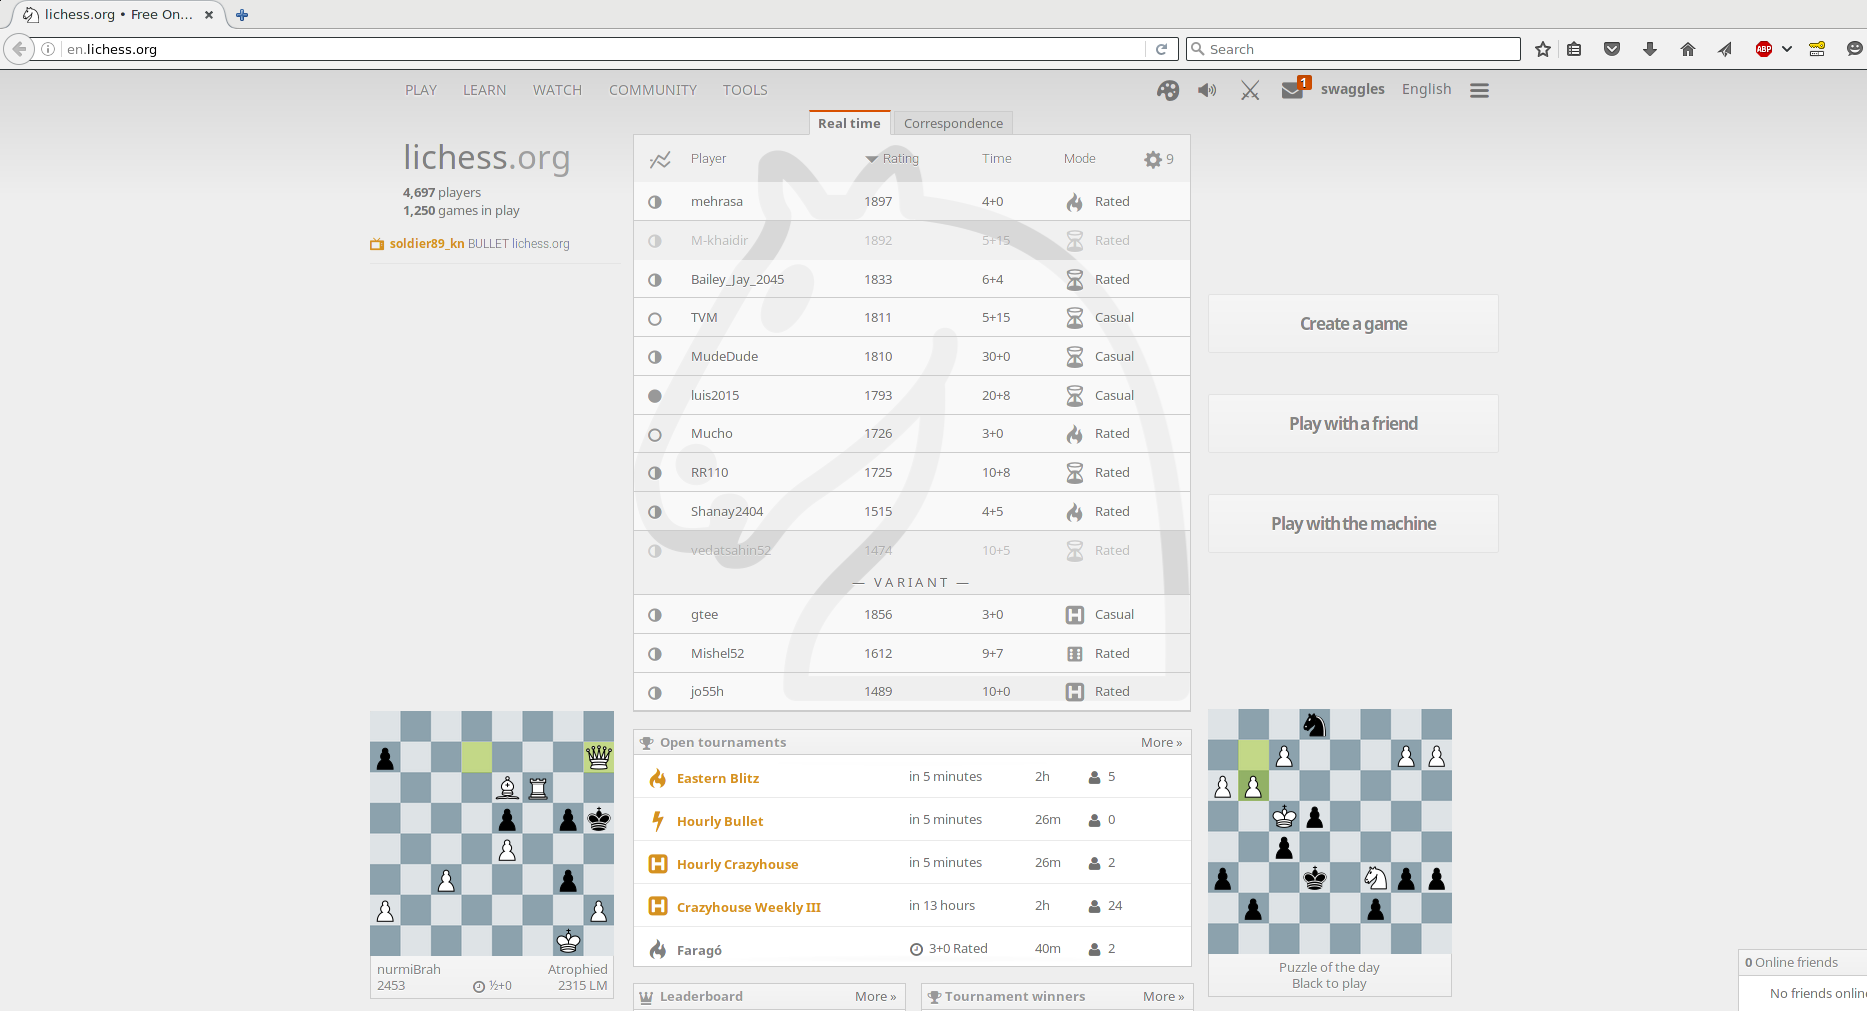
\includegraphics[height=0.4\textheight,natwidth=1867,natheight=1011]{image/lichess.png}
\end{block}
\end{frame}

\begin{frame}[fragile]
\frametitle{The Expression Problem}
\begin{block}{Cheat Detection}
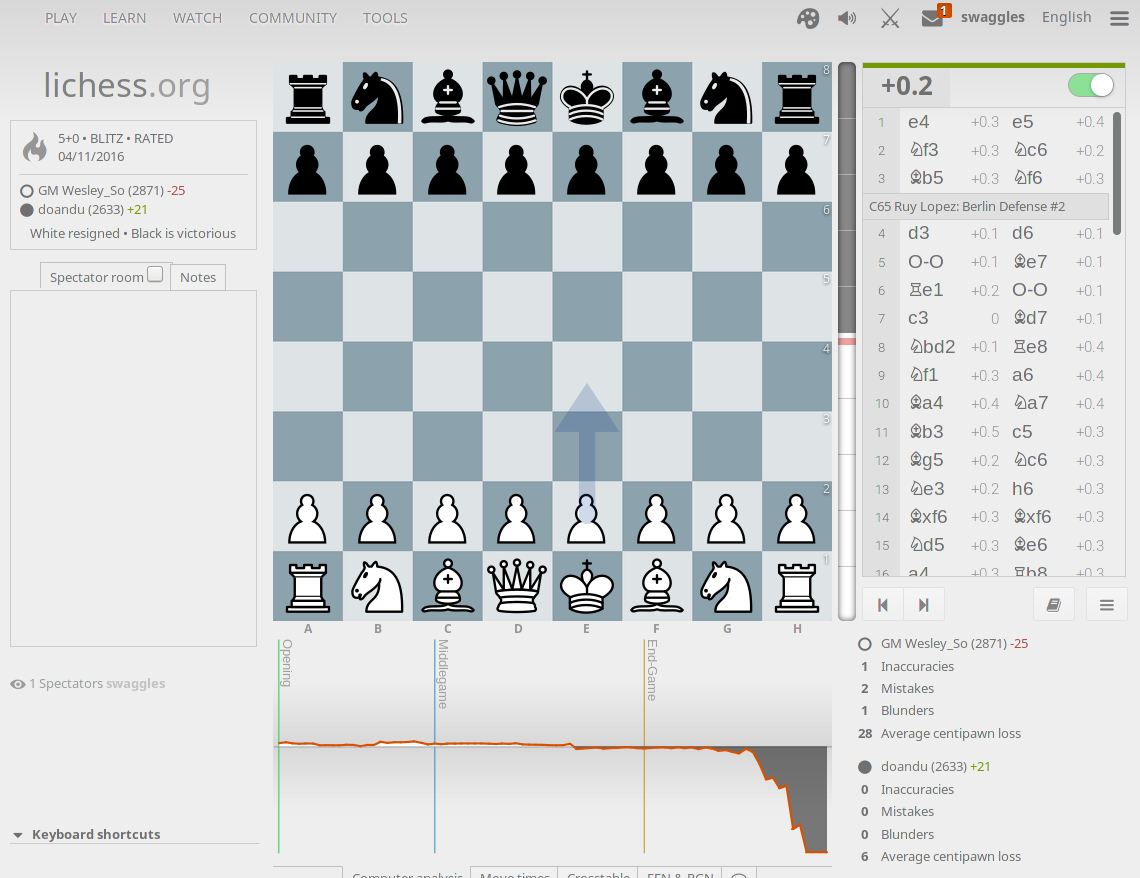
\includegraphics[height=0.5\textheight,natwidth=1140,natheight=878]{image/lichess-wesley-so.png}
\par
Here is the world \#12 being beaten by a patzer using computer-assistance.
\end{block}
\end{frame}

\begin{frame}[fragile]
\frametitle{The Expression Problem}
\begin{block}{Cheat Detection}

\includegraphics[height=0.2\textheight,natwidth=883,natheight=184]{image/lichess-wesley-so-announce.png}
\par
Here is the world \#12 being beaten by a patzer using computer-assistance.
\end{block}
\end{frame}

\begin{frame}[fragile]
\frametitle{The Expression Problem}
\begin{block}{An incidental advantage}
GPS Exchange Format (GPX) is the open standard format for GPS tracks,
waypoints and routes.
\end{block}
\end{frame}

\begin{frame}[fragile]
\frametitle{The Expression Problem}
\begin{block}{An incidental advantage}
\begin{itemize}
\item a \textbf{gpx} has zero or many \textbf{tracks}
\item a \textbf{track} has zero or many \textbf{segments}
\item a \textbf{segment} has zero or many \textbf{track points}
\item a \textbf{track point} has one \textbf{latitude}
\item a \textbf{latitude} has a \textbf{decimal value between} -90 and 90
\end{itemize}
\end{block}
\end{frame}

\begin{frame}[fragile]
\frametitle{The Expression Problem}
\begin{block}{An incidental advantage}
\begin{lstlisting}[style=haskell,mathescape]
gpxTrack =
  _Gpx . _Track
gpxTrackSegment =
  _GpxTrack . _Segment
gpxTrackSegmentTrackPointLatitude =
  _GpxTrackSegment . _TrackPoint . _Latitude
\end{lstlisting}
\end{block}
\end{frame}

\begin{frame}[fragile]
\frametitle{The Expression Problem}
\begin{block}{An incidental advantage}
\begin{lstlisting}[style=haskell,mathescape]
instance AsLatitude Gpx where $\ldots$
\end{lstlisting}
No need to come up with a tree of identifier names!
\end{block}
\end{frame}


\begin{frame}[fragile]
\frametitle{The Expression Problem}
\begin{block}{Disadvantages}
What are some of the penalties?
\end{block}
\end{frame}

\begin{frame}[fragile]
\frametitle{The Expression Problem}
\begin{block}{Disadvantages}
Lots of boilerplate
\begin{itemize}
\item \lstinline[style=haskell, mathescape]{ $\{$-# LANGUAGE MultiParamTypeClasses, FlexibleInstances #-$\}$ }
\item A type-class.
\item An equivalence instance \lstinline[style=haskell]{(id)}.
\item The instance for the field or constructor.
\end{itemize}
\end{block}
\end{frame}

\begin{frame}[fragile]
\frametitle{The Expression Problem}
\begin{block}{Disadvantages}
Type errors are difficult to navigate.
\begin{lstlisting}[style=haskell,mathescape]
$\lambda$> 12.34 .#. 56.78

No instance for (Fractional lat0)
      arising from the literal '12.34'
The type variable 'lat0' is ambiguous

No instance for (AsLongitude
      (->) (Control.Applicative.Const Longitude) lon0)
  arising from a use of '.#.'
\end{lstlisting}
\end{block}
\end{frame}

\begin{frame}[fragile]
\frametitle{The Expression Problem}
\begin{block}{Disadvantages}
Type \textbf{signatures} are difficult to navigate.
\begin{lstlisting}[style=haskell,basicstyle=\tiny,mathescape]
javaClassFileParser ::
  (AsEmpty (c Word8), AsEmpty (t Char),
    AsEmpty (f (Attribute a1)), AsEmpty (a Word8),
    AsEmpty (m (Attribute a2)), AsEmpty (a3 Word8), AsEmpty (a4 Word8),
    AsEmpty (c1 (ConstantPoolInfo p)), AsEmpty (i Word16),
    AsEmpty (s1 (Field a5 f1)), AsEmpty (t1 (Method m1 b)),
    AsEmpty (u (Attribute d)), Cons (c Word8) (c Word8) Word8 Word8,
    Cons (t Char) (t Char) Char Char,
    Cons
      (f (Attribute a1)) (f (Attribute a1)) (Attribute a) (Attribute a),
    Cons (a Word8) (a Word8) Word8 Word8,
    Cons
      (m (Attribute a2))
      (m (Attribute a2))
      (Attribute a3)
      (Attribute a3),
    Cons (a3 Word8) (a3 Word8) Word8 Word8,
    Cons (a4 Word8) (a4 Word8) Word8 Word8,
    Cons
      (c1 (ConstantPoolInfo p))
      (c1 (ConstantPoolInfo p))
      (ConstantPoolInfo t)
      (ConstantPoolInfo t),
    Cons (i Word16) (i Word16) Word16 Word16,
    $\ldots$
\end{lstlisting}
\end{block}
\end{frame}

\begin{frame}[fragile]
\frametitle{The Expression Problem}
\begin{block}{Disadvantages}
No, srsly.
\begin{lstlisting}[style=haskell,basicstyle=\tiny,mathescape]
    $\ldots$
    Cons
      (s1 (Field a5 f1)) (s1 (Field a5 f1)) (Field a1 f) (Field a1 f),
    Cons
      (t1 (Method m1 b)) (t1 (Method m1 b)) (Method m a2) (Method m a2),
    Cons
      (u (Attribute d)) (u (Attribute d)) (Attribute a4) (Attribute a4),
    AsClassFileCafebabeError Tagged Identity (s c),
    AsClassFileVersionError Tagged Identity (s c),
    AsClassFileConstantPoolError Tagged Identity s,
    AsClassFileThisAccessFlagsError Tagged Identity (s c),
    AsClassFileThisClassError Tagged Identity (s c),
    AsClassFileSuperClassError Tagged Identity (s c),
    AsClassFileInterfacesError Tagged Identity (s c),
    AsClassFileFieldsError Tagged Identity (s c),
    AsClassFileMethodsError Tagged Identity (s c),
    AsClassFileAttributesError Tagged Identity (s c),
    AsClassFileUnexpectedInputOnStream Tagged Identity (s c)) =>
  Get (s c) (ClassFile p c1 i a5 f1 s1 m1 b t1 d u)
\end{lstlisting}
\end{block}
\end{frame}

\begin{frame}[fragile]
\frametitle{The Expression Problem}
\begin{block}{Disadvantages}
However,
\begin{itemize}
\item This java class file parser works for both version 1.5 and 1.7 class files.
\item Works for future java versions.
\item Derived functions work against similar formats (.NET).
\item and I can prove all this by \textbf{parametricity}.
\end{itemize}
\end{block}
\end{frame}

\begin{frame}
\frametitle{Conclusion}
\begin{block}{Discussion}
\begin{itemize}
\item<1-> The Expression Problem has been conquered in part by exploiting lens abstractions.
\item<2-> For real this time; with demonstrable benefits.
\item<3-> However, there are penalties.
\item<4-> Is there an even better way?
\end{itemize}
\end{block}
\end{frame}

\begin{frame}
\frametitle{References}

\bibliographystyle{amsalpha}
\bibliography{tep-lens}

\end{frame}


\end{document}
